\chapter{Organogénesis: la construcción de la extremidad de los tetrápodos}\label{ch:b2:limb-organogenesis}

Tres días después de la puesta de un huevo de gallina aparece a cada lado
del embrión un abultamiento del tamaño de una cabeza de alfiler. Cuatro
días más tarde es un ala, con un húmero, un radio y un cúbito, una muñeca y
tres dedos, en el orden correcto, con las longitudes correctas y con los
músculos unidos a los huesos correctos. Si se corta el reborde de piel
engrosada del abultamiento, el ala deja de crecer; si se injerta una
lámina de su margen posterior en el anterior, crecen seis dedos en imagen
especular. El \omterm{def:b2:limb-organogenesis:bud}{esbozo de la extremidad} es el caso clásico de
\emph{organogénesis} --- la construcción de un órgano a partir de un
campo de células mediante señales que indican a cada célula a qué
distancia está hacia fuera, hacia delante y hacia arriba ---, y los
experimentos que la descifraron están entre los más claros de la
biología. Este capítulo sigue el esbozo desde su crecimiento hasta su
esqueleto.

\section{El esbozo y sus tres ejes}

\begin{definition}[El esbozo de la extremidad]\label{def:b2:limb-organogenesis:bud}
\index{esbozo de la extremidad}\index{cresta ectodérmica apical}\index{zona de actividad polarizante}
El \emph{esbozo de la extremidad} es un abultamiento de \emph{mesodermo de
la lámina lateral} cubierto de ectodermo, que surge en una posición fija a
lo largo del flanco (el \emph{campo de la extremidad}) donde lo permite el
código Hox del eje corporal; su mesodermo formará hueso, cartílago,
tendón y dermis, y las células que migran a él desde los somitos formarán
los músculos. El esbozo tiene tres ejes, cada uno gobernado por un centro
de señalización. \emph{Proximodistal} (del hombro a la punta de los
dedos): la \emph{cresta ectodérmica apical} (AER), una franja engrosada de
ectodermo a lo largo del extremo, secreta \omterm{prop:b2:limb-organogenesis:aer}{factores de crecimiento de
fibroblastos} (FGF) que mantienen en división y sin diferenciar el
mesodermo situado debajo. \emph{Anteroposterior} (del pulgar al meñique):
la \emph{zona de actividad polarizante} (ZPA), un bloque de mesodermo en
el margen posterior, secreta el morfógeno \emph{\omterm{prop:b2:limb-organogenesis:zpa}{Sonic hedgehog}} (Shh).
\emph{Dorsoventral} (del dorso de la mano a la palma): el ectodermo dorsal
secreta Wnt7a. Los esbozos de las extremidades anteriores y posteriores
son parecidos y usan las mismas señales; difieren en un factor de
transcripción expresado antes de que aparezca el esbozo (Tbx5 en la
extremidad anterior, Tbx4 en la posterior), y por eso un ala es un ala.
\end{definition}

\begin{omfigure}
\begin{tikzpicture}[every node/.style={font=\scriptsize}, >=stealth]
  % flank
  \fill[omExo!25] (0,-2.2) rectangle (1.2,2.2); \node[rotate=90] at (0.6,0) {pared corporal (flanco)};
  % bud outline: paddle
  \draw[thick, fill=omDef!10] (1.2,1.4) .. controls (3.0,1.9) and (5.2,1.6) .. (5.8,0.3) .. controls (5.9,-0.3) and (5.2,-1.6) .. (3.4,-1.7) .. controls (2.4,-1.8) and (1.6,-1.5) .. (1.2,-1.4);
  % AER along the tip
  \draw[line width=3pt, omThm] (5.2,1.3) .. controls (5.9,0.6) and (5.9,-0.6) .. (5.0,-1.4);
  \node[omThm, anchor=west, align=left] at (6.1,0.9) {cresta ectodérmica apical (AER):\\FGF, crecimiento proximodistal};
  % ZPA posterior
  \draw[thick, omProp, fill=omProp!50] (2.4,-1.1) ellipse (0.55 and 0.4);
  \draw[omProp] (2.4,-1.5) -- (2.4,-2.0);
  \node[omProp, anchor=north, align=center] at (2.6,-2.0) {ZPA (margen posterior):\\Sonic hedgehog, anteroposterior};
  % dorsal ectoderm
  \draw[line width=2pt, omDef!70!black] (1.4,1.55) .. controls (3.0,2.0) and (5.0,1.7) .. (5.4,1.2);
  \node[omDef!70!black, anchor=south] at (3.4,2.05) {ectodermo dorsal: Wnt7a, dorsoventral};
  % axes
  \draw[->, thick] (1.5,-3.1) -- (5.5,-3.1); \node[below] at (3.5,-3.15) {proximal $\to$ distal};
  \draw[->, thick] (10.6,-1.6) -- (10.6,1.2); \node[right, align=left] at (10.7,-0.2) {posterior $\to$ anterior\\(del meñique al pulgar)};
\end{tikzpicture}

{\small El \omterm{def:b2:limb-organogenesis:bud}{esbozo de la extremidad} del pollo visto desde arriba, con sus
tres centros de señalización: la AER a lo largo del extremo impulsa el
crecimiento, la ZPA en el margen posterior organiza los dedos y el
ectodermo dorsal distingue el dorso de la palma.}
\end{omfigure}

\begin{omfigure}
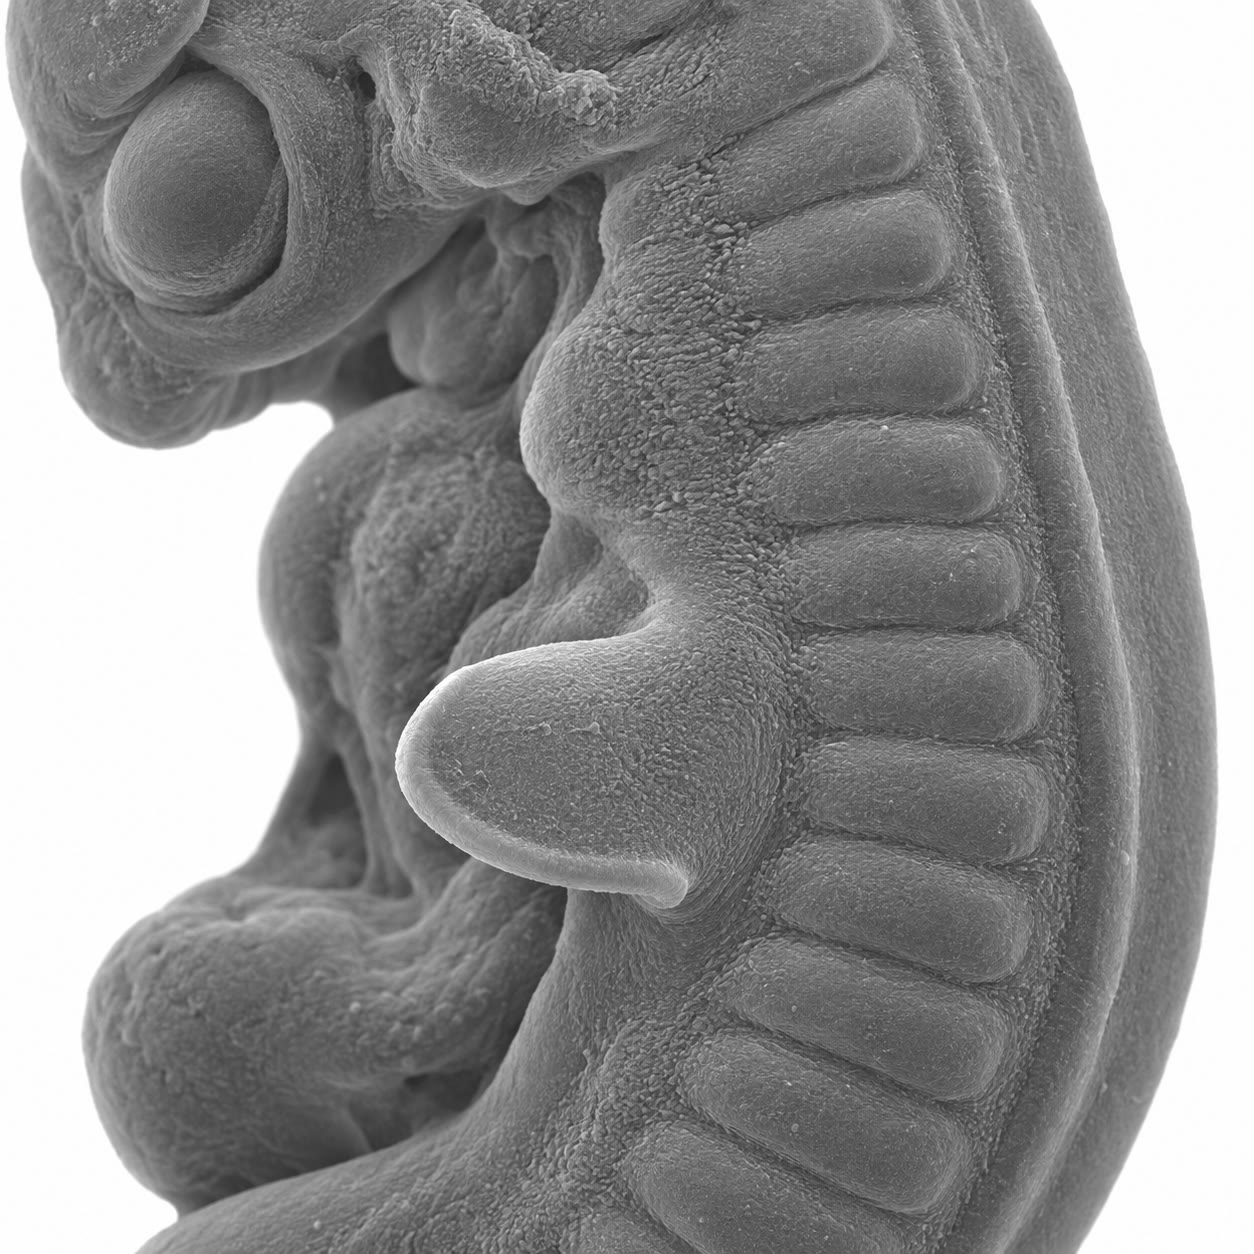
\includegraphics[width=0.42\linewidth]{images/book4/ai/b4-11-limb-bud.jpg}

{\small Un embrión de pollo al microscopio electrónico de barrido: la
hilera de somitos a lo largo del tronco y, en el flanco, el \omterm{def:b2:limb-organogenesis:bud}{esbozo de la
extremidad} en forma de pala, con la cresta engrosada a lo largo de su
borde.}
\end{omfigure}

\section{El crecimiento: el eje proximodistal}

\begin{proposition}[La cresta ectodérmica apical]\label{prop:b2:limb-organogenesis:aer}
\index{factor de crecimiento de fibroblastos}\index{zona de progreso}
La AER es necesaria para el crecimiento, y sus FGF son suficientes: el
mesodermo situado debajo, la \emph{\omterm{prop:b2:limb-organogenesis:aer}{zona de progreso}}, se divide
aproximadamente cada doce horas, y las células que abandonan la zona a
medida que avanza el extremo dejan de dividirse, se condensan y se
diferencian. El esqueleto se forma en orden proximodistal ---
\emph{estilopodio} (húmero o fémur), \emph{zeugopodio} (radio y cúbito,
tibia y peroné), \emph{autopodio} (muñeca y dedos) ---, cada segmento
especificado a su vez a medida que crece el esbozo, y los segmentos se
corresponden con dominios anidados de expresión de genes Hox (Hoxa/d
9--10 en el estilopodio, 11 en el zeugopodio, 13 en el autopodio). Un
esbozo de extremidad multiplica su longitud por unas diez veces en cuatro
días mientras el alcance de la señal de la cresta se mantiene en los
mismos pocos cientos de micrómetros, de modo que la cresta no organiza la
extremidad de una vez sino como un frente móvil, como una impresora que
imprime una página línea a línea.
\end{proposition}
\begin{proof}[Evidencia]
Saunders (1948) extirpó la AER de esbozos de ala de pollo en estadios
sucesivos: extirpada pronto, el esbozo solo dio un muñón de húmero;
extirpada un día más tarde, húmero y antebrazo, pero sin mano; extirpada
aún más tarde, un ala casi completa --- cuanto más tardía la operación,
más distal el nivel de truncamiento, de modo que la cresta es necesaria
para cada segmento sucesivamente. El injerto de una segunda cresta
produjo un segundo crecimiento; una bola impregnada de FGF, colocada en un
esbozo al que se había extirpado la cresta, restableció una extremidad
completa (Niswander, 1993), y una bola colocada en el flanco entre los
campos de las extremidades indujo una extremidad adicional. Los ratones
que carecen de los FGF de la cresta no tienen extremidades.
\end{proof}

\begin{omfigure}
\begin{tikzpicture}[every node/.style={font=\scriptsize}]
  \foreach \x/\lab/\n in {0/{AER extirpada pronto:\\solo húmero}/1, 3.6/{extirpada un día después:\\húmero, radio, cúbito}/2, 7.2/{extirpada aún más tarde:\\ala casi completa}/3, 10.8/{intacta:\\ala completa}/4} {
    \begin{scope}[xshift=\x cm]
      \fill[omExo!25] (0,-0.5) rectangle (0.5,2.6);
      % humerus
      \draw[thick, fill=omDef!25, rounded corners=3pt] (0.6,0.9) rectangle (1.7,1.2);
      \ifnum\n>1 \draw[thick, fill=omDef!25, rounded corners=3pt] (1.8,1.05) rectangle (2.7,1.3); \draw[thick, fill=omDef!25, rounded corners=3pt] (1.8,0.75) rectangle (2.7,1.0); \fi
      \ifnum\n>2 \foreach \y in {0.55,0.85,1.15} \draw[thick, fill=omDef!25, rounded corners=2pt] (2.8,\y) rectangle (3.3,\y+0.2); \fi
      \ifnum\n=4 \foreach \y in {0.55,0.85,1.15} \draw[thick, fill=omDef!25, rounded corners=2pt] (3.35,\y) rectangle (3.5,\y+0.2); \fi
      \node[below, align=center] at (1.8,-0.2) {\lab};
    \end{scope}
  }
\end{tikzpicture}

{\small El experimento de Saunders. Cuanto antes se extirpa la cresta,
más parte de la extremidad falta, siempre desde el extremo: la cresta es
necesaria para cada segmento mientras ese segmento se está formando.}
\end{omfigure}

\begin{theorem}[El crecimiento por división]\label{thm:b2:limb-organogenesis:growth}
Un esbozo cuyas células se dividen cada $T$ horas multiplica su número de
células por $2^{t/T}$ en un tiempo $t$; cuatro días de ciclos de doce
horas dan
$2^{8} = 256$. Si el volumen del esbozo se multiplica por mil en esos
cuatro días, la división aporta un factor 256 y el factor cuatro restante
debe proceder del aumento de tamaño de las células y de la matriz que las
células del cartílago secretan a su alrededor. A la inversa, un segmento
que tarda un ciclo celular en especificarse --- las doce horas
aproximadamente que separan los sucesivos niveles de truncamiento del
experimento de Saunders --- corresponde a una duplicación de la \omterm{prop:b2:limb-organogenesis:aer}{zona de
progreso}.
\end{theorem}
\begin{proof}
$N(t) = N_0 2^{t/T}$; con $t = \qty{96}{h}$ y $T = \qty{12}{h}$,
$t/T = 8$. La razón entre el factor necesario y el factor aportado por la
división, $1000/256 \approx 4$, es lo que debe aportar el crecimiento
distinto de la división.
\end{proof}

\section{Los dedos: el eje anteroposterior}
\section{Los dedos: el eje anteroposterior}

\begin{proposition}[La zona de actividad polarizante]\label{prop:b2:limb-organogenesis:zpa}
\index{Sonic hedgehog}\index{morfógeno!Shh}
La ZPA especifica qué dedo se forma y dónde. Sus células secretan \omterm{prop:b2:limb-organogenesis:zpa}{Sonic
hedgehog}, que se extiende por el esbozo desde el margen posterior, y las
células del mesodermo leen la concentración --- y el tiempo durante el
que han estado expuestas a ella --- como una posición: la dosis más alta
da el dedo más posterior; las dosis menores, dedos más anteriores; y por
debajo de un umbral no se forma ningún dedo. El gradiente tiene la forma
exponencial del \cref{ch:b2:vertebrate-development}, con una longitud de
decaimiento de unas pocas decenas de micrómetros, y sus umbrales dividen
el esbozo en los primordios de los dedos: en el ala del pollo, de
posterior a anterior, los dedos 4, 3 y 2. Una segunda fuente de la señal
en el margen anterior produce un segundo juego, en imagen especular; una
fuente más débil, o una exposición más corta, solo produce los dedos
anteriores del juego adicional. El mismo gen, con la misma función,
organiza los dedos de todos los tetrápodos, y una \omterm{def:b2:genome-diversification:mutation}{mutación} que añade una
fuente anterior de Shh da polidactilia en gatos, pollos, ratones y
personas.
\end{proposition}
\begin{proof}[Evidencia]
Saunders y Gasseling (1968) injertaron un bloque de mesodermo del margen
posterior de un esbozo de ala de pollo en el margen anterior de otro: el
huésped desarrolló un ala con seis dedos en el orden 4-3-2-2-3-4, una
imagen especular respecto al centro. Tickle (1975) mostró que el número de
dedos adicionales dependía del número de células injertadas --- una
dosis. Riddle y Tabin (1993) descubrieron que el tejido injertado
expresaba el gen \emph{\omterm{prop:b2:limb-organogenesis:zpa}{Sonic hedgehog}}, que el gen no se expresaba en
ninguna otra parte del esbozo, y que células modificadas para expresarlo,
injertadas en posición anterior, reproducían la duplicación especular;
una bola de la proteína hacía lo mismo. Los pollos mutantes con una zona
ectópica anterior de Shh tienen dedos anteriores adicionales.
\end{proof}

\begin{omfigure}
\begin{tikzpicture}[every node/.style={font=\scriptsize}, >=stealth]
  % normal bud with gradient and digits
  \begin{scope}
    \fill[omExo!25] (0,-0.3) rectangle (0.4,3.3);
    \shade[bottom color=omProp!60, top color=white] (0.4,-0.3) rectangle (3.2,3.3);
    \draw[thick] (0.4,-0.3) rectangle (3.2,3.3);
    \draw[thick, omProp, fill=omProp!70] (0.9,0.1) ellipse (0.45 and 0.35); \node[omProp!80!black, anchor=west] at (1.4,0.1) {ZPA};
    \foreach \y/\d in {0.6/4, 1.5/3, 2.4/2} { \draw[thick, fill=omDef!25, rounded corners=2pt] (3.3,\y-0.12) rectangle (4.2,\y+0.12); \node[right] at (4.25,\y) {dedo \d}; }
    \node[below, align=center] at (2.0,-0.5) {esbozo normal: Shh desde el\\margen posterior, dedos 4-3-2};
    \draw[->, thick] (-0.4,0.2) -- (-0.4,3.0); \node[rotate=90] at (-0.7,1.6) {posterior $\to$ anterior};
  \end{scope}
  % grafted bud
  \begin{scope}[xshift=7cm]
    \fill[omExo!25] (0,-0.3) rectangle (0.4,3.3);
    \shade[bottom color=omProp!60, top color=white] (0.4,-0.3) rectangle (3.2,1.5);
    \shade[top color=omProp!60, bottom color=white] (0.4,1.5) rectangle (3.2,3.3);
    \draw[thick] (0.4,-0.3) rectangle (3.2,3.3);
    \draw[thick, omProp, fill=omProp!70] (0.9,0.1) ellipse (0.45 and 0.35);
    \draw[thick, omProp, fill=omProp!70] (0.9,2.9) ellipse (0.45 and 0.35); \node[omProp!80!black, anchor=west] at (1.4,2.9) {ZPA injertada};
    \foreach \y/\d in {0.3/4, 0.8/3, 1.3/2, 1.7/2, 2.2/3, 2.7/4} { \draw[thick, fill=omDef!25, rounded corners=2pt] (3.3,\y-0.1) rectangle (4.2,\y+0.1); \node[right] at (4.25,\y) {\d}; }
    \node[below, align=center] at (2.0,-0.5) {ZPA injertada en posición anterior:\\duplicación especular 4-3-2-2-3-4};
  \end{scope}
\end{tikzpicture}

{\small La región polarizante. Izquierda: Shh se extiende desde el margen
posterior y su concentración decreciente especifica los dedos 4, 3 y 2.
Derecha: una segunda ZPA injertada en el margen anterior crea un segundo
gradiente y un juego de dedos en imagen especular.}
\end{omfigure}

\begin{theorem}[Las fronteras de los dedos a partir del gradiente]\label{thm:b2:limb-organogenesis:thresholds}
Con Shh a una concentración $c_0$ en el margen posterior y una longitud de
decaimiento $\lambda$, la frontera del territorio de un dedo cuyo umbral
es $T_i$ se sitúa a $x_i = \lambda\ln(c_0/T_i)$ del margen. Con
$\lambda = \qty{50}{\micro m}$ y umbrales de $0.6$,
$0.25$ y $0.08$ de $c_0$ para los dedos 4, 3 y 2, los territorios
son $0$--$26$, $26$--$69$ y $69$--$126$ micrómetros, y el tejido situado
más allá de \qty{126}{\micro m} no forma ningún dedo. Duplicar la fuente
desplaza cada frontera hacia fuera en $\lambda\ln 2 = \qty{35}{\micro m}$
--- suficiente, en un esbozo de unos pocos cientos de micrómetros, para
añadir un dedo en el borde anterior; una segunda fuente en el margen
anterior dispone los mismos territorios en orden inverso.
\end{theorem}
\begin{proof}
A partir de $c(x) = c_0 e^{-x/\lambda}$, $c = T_i$ en $x_i = \lambda
\ln(c_0/T_i)$: $50\ln(1/0.6) = 25.5$, $50\ln 4 = 69$, $50\ln 12.5 =
126$. Sustituir $c_0$ por $2c_0$ suma $\lambda\ln 2$ a cada $x_i$.
\end{proof}

\begin{omfigure}
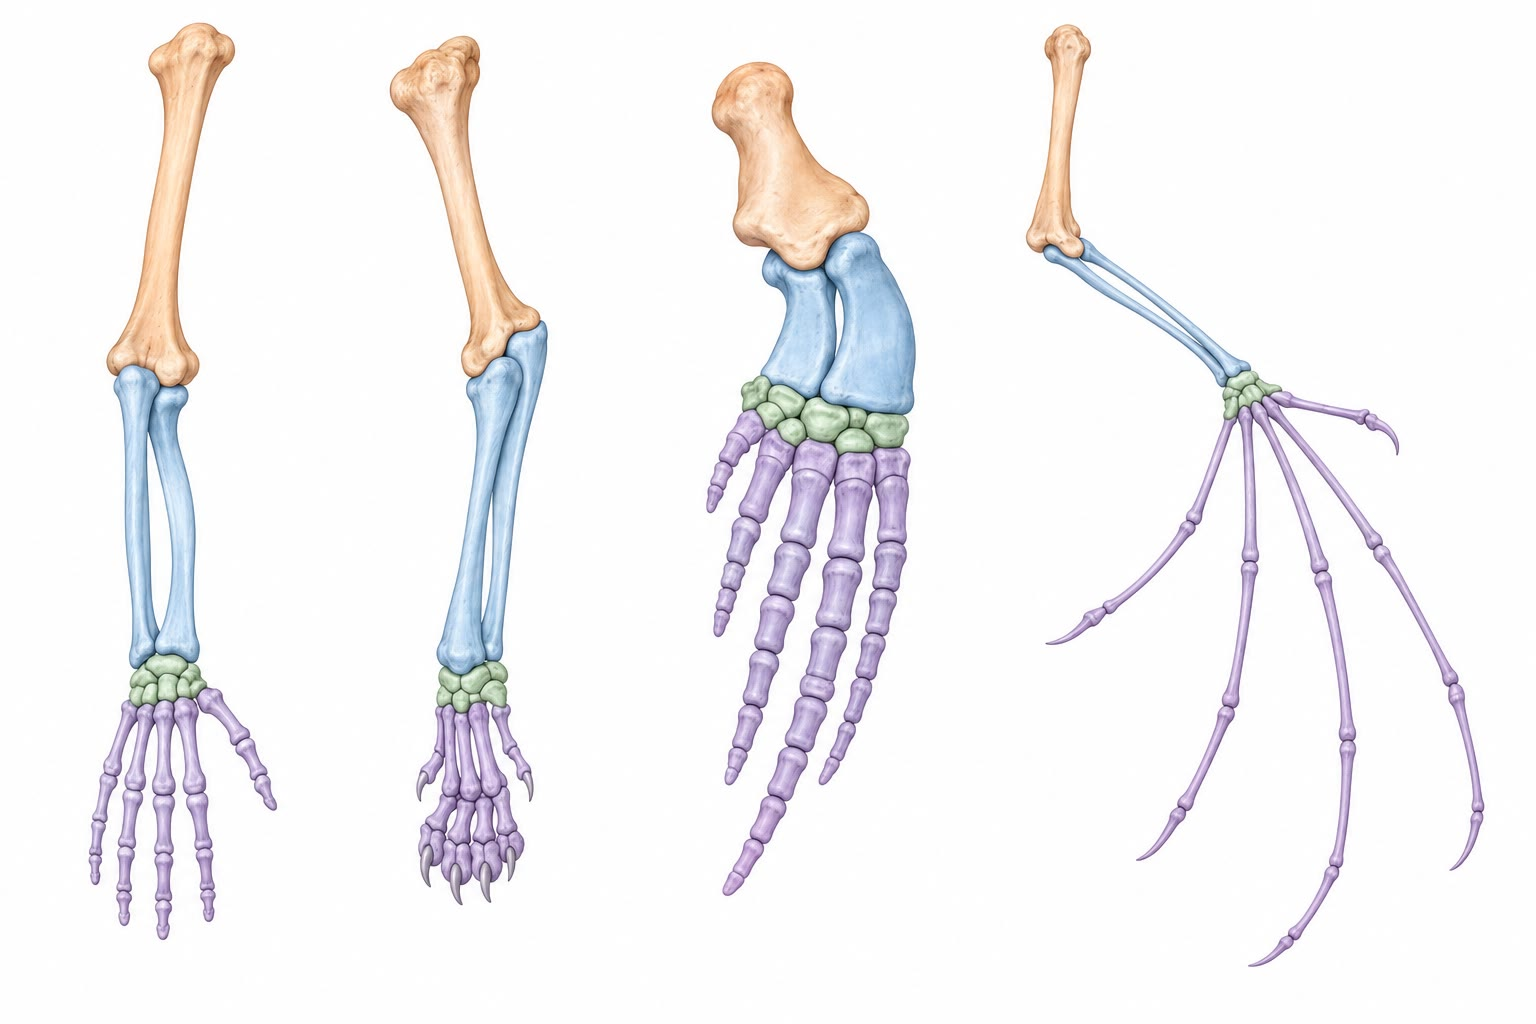
\includegraphics[width=0.66\linewidth]{images/book4/ai/b4-11-tetrapod-limbs.jpg}

{\small Un plan, cuatro extremidades: las extremidades anteriores de un
ser humano, un gato, una ballena y un murciélago comparten los mismos
huesos en el mismo orden --- un estilopodio, dos huesos del zeugopodio,
la muñeca, los dedos ---, construidos por los mismos centros de
señalización y distintos en su crecimiento.}
\end{omfigure}

\section{Coordinación y modelado}

\begin{proposition}[Los ejes se comunican entre sí]\label{prop:b2:limb-organogenesis:loop}
\index{bucle de retroalimentación!del desarrollo}
Los centros se mantienen mutuamente: el FGF de la cresta mantiene la
expresión de Shh en la ZPA, y Shh, a través de un relevo en el mesodermo,
mantiene la expresión de FGF en la cresta; si se elimina uno, el otro se
apaga en un día. El Wnt7a del ectodermo dorsal también es necesario para
la expresión completa de Shh, y dirige el destino dorsal del mesodermo
(un ratón que carece de él tiene dos palmas). Esta dependencia mutua es un
\emph{bucle de retroalimentación positiva} que acopla los tres ejes: la
extremidad solo crece donde se está organizando, y solo se organiza donde
está creciendo, de modo que un esbozo nunca forma una mano sin brazo ni
dedos del tipo equivocado. Cuando el crecimiento termina, el bucle se
rompe --- el mesodermo deja de hacer de relevo, Shh se detiene, la cresta
regresa --- y la extremidad deja de crecer en su tamaño propio.
\end{proposition}

\begin{proposition}[Del patrón al hueso]\label{prop:b2:limb-organogenesis:skeleton}
\index{condrogénesis}\index{apoptosis!interdigital}
Una vez especificadas, las células del mesodermo que abandonan la \omterm{prop:b2:limb-organogenesis:aer}{zona de
progreso} se \emph{condensan} en varillas y placas con la forma de los
futuros huesos, se diferencian en células de cartílago que secretan una
matriz rica en colágeno y proteoglucanos, y construyen un modelo
cartilaginoso de cada elemento esquelético; las articulaciones se forman
donde una banda de células recibe la orden de no convertirse en
cartílago; los vasos sanguíneos invaden los modelos y el hueso sustituye
al cartílago desde el centro hacia fuera, dejando en los extremos unas
placas de crecimiento que mantienen el alargamiento del hueso hasta la
edad adulta (\emph{osificación endocondral}). Los precursores musculares
de los somitos migran hacia la extremidad, se dividen, se fusionan en
fibras
(\cref{ch:b2:cell-differentiation}) y se unen mediante tendones formados
por el propio mesodermo de la extremidad. Entre los radios de los dedos,
el tejido se elimina por muerte celular programada: las células de las
membranas interdigitales, instruidas por una señal de proteína
morfogenética ósea (BMP), activan su propia destrucción y son eliminadas
en un día, lo que separa los dedos. Un pato conserva sus membranas porque
en su tejido interdigital se expresa un inhibidor de la BMP; un pollo al
que se aplica ese inhibidor en una bola desarrolla patas palmeadas.
\end{proposition}
\begin{proof}[Evidencia]
El mesodermo interdigital cortado de un esbozo de pata de pollo e
injertado en otro lugar muere según lo previsto --- la muerte es
intrínseca, decidida antes de que se extraiga el tejido; el mismo tejido
de un pato sobrevive. Unas bolas de BMP colocadas entre los dedos de un
pato hacen morir la membrana; unas bolas del inhibidor gremlin colocadas
entre los dedos de un pollo la salvan. Un ratón que carece de un receptor
de BMP en la extremidad conserva sus membranas.
\end{proof}

\begin{omfigure}
\begin{tikzpicture}[every node/.style={font=\scriptsize}]
  \foreach \x/\lab in {0/{los radios de los dedos se\\condensan como cartílago}, 4.2/{las células interdigitales\\mueren (BMP)}, 8.4/{dedos separados; el hueso\\sustituye al cartílago}} {
    \begin{scope}[xshift=\x cm]
      \node[below, align=center] at (1.5,-0.3) {\lab};
    \end{scope}
  }
  % stage 1: paddle with rays
  \draw[thick, fill=omDef!8] (0,0) .. controls (0,2.2) and (3,2.2) .. (3,0) -- cycle;
  \foreach \x in {0.6,1.2,1.8,2.4} \draw[thick, fill=omDef!30, rounded corners=2pt] (\x-0.12,0.1) rectangle (\x+0.12,1.5);
  % stage 2: paddle with dying webs
  \begin{scope}[xshift=4.2cm]
    \draw[thick, fill=omDef!8] (0,0) .. controls (0,2.2) and (3,2.2) .. (3,0) -- cycle;
    \foreach \x in {0.6,1.2,1.8,2.4} \draw[thick, fill=omDef!30, rounded corners=2pt] (\x-0.12,0.1) rectangle (\x+0.12,1.5);
    \foreach \x in {0.9,1.5,2.1} \foreach \y in {0.7,1.0,1.3} \fill[omThm] (\x,\y) circle (0.05);
  \end{scope}
  % stage 3: separated digits
  \begin{scope}[xshift=8.4cm]
    \draw[thick, fill=omDef!8] (0,0) -- (0,0.5) -- (0.3,0.5) -- (0.35,1.7) -- (0.85,1.7) -- (0.9,0.5) -- (1.05,0.5) -- (1.1,1.85) -- (1.6,1.85) -- (1.65,0.5) -- (1.8,0.5) -- (1.85,1.7) -- (2.35,1.7) -- (2.4,0.5) -- (2.7,0.5) -- (2.7,0) -- cycle;
    \foreach \x in {0.6,1.35,2.1} \draw[thick, fill=omExo!60, rounded corners=2pt] (\x-0.1,0.1) rectangle (\x+0.1,1.4);
  \end{scope}
\end{tikzpicture}

{\small El modelado de la mano: los radios cartilaginosos se condensan en
la pala, las células que hay entre ellos mueren (rojo) y los dedos
liberados se osifican.}
\end{omfigure}

\begin{example}[La misma extremidad, con otro crecimiento]\label{ex:b2:limb-organogenesis:evolution}
El ala del murciélago es una mano cuyos dedos 2 a 5 crecieron varias veces
más que los de un ratón --- un potenciador de un gen de la extremidad,
trasplantado del murciélago al ratón, alarga los huesos de la extremidad
anterior del ratón --- y cuyo tejido interdigital sobrevivió, porque la
membrana expresa el inhibidor de la BMP que usa el pato. La aleta de la
ballena es una mano con falanges adicionales y sin muerte interdigital.
La pata del caballo es un solo dedo con los demás reducidos a estiletes.
La serpiente no tiene extremidades porque su flanco nunca expresa las
señales que inician un esbozo. Y las aletas de los peces, que carecen de
autopodio, las construyen la misma AER y la misma ZPA, pero detienen su
programa Hox antes de la fase tardía que forma los dedos; el fósil
\emph{Tiktaalik} (de 375 millones de años) muestra la aparición de la
muñeca en una aleta. La evolución de las extremidades es sobre todo la
modulación de un programa conservado --- cuánto dura cada fase, hasta
dónde llega cada señal, qué células mueren.
\end{example}

\section{Ejercicios}

\begin{exercise}[$\star$]\label{exo:b2:limb-organogenesis:1}
Nómbrense los tres ejes del \omterm{def:b2:limb-organogenesis:bud}{esbozo de la extremidad} y, para cada uno, el
centro de señalización, su posición y su señal.
\end{exercise}

\begin{exercise}[$\star$]\label{exo:b2:limb-organogenesis:2}
Dense los tres segmentos del esqueleto de la extremidad y los huesos de
cada uno en un brazo y una pierna humanos. ¿Qué genes Hox los marcan?
\end{exercise}

\begin{exercise}[$\star$]\label{exo:b2:limb-organogenesis:3}
Enumérense, por orden, las etapas que llevan de una zona de mesodermo de
la lámina lateral a un dedo con su hueso, su articulación y su músculo.
\end{exercise}

\begin{exercise}[$\star$]\label{exo:b2:limb-organogenesis:4}
¿Qué aspecto tiene la extremidad si la AER se extirpa (a) en cuanto
aparece el esbozo, (b) después de que se haya especificado el antebrazo,
(c) no se extirpa sino que se sustituye por una bola de FGF?
\end{exercise}

\begin{exercise}[$\star\star$]\label{exo:b2:limb-organogenesis:5}
Con $\lambda = \qty{40}{\micro m}$ y umbrales de $0.5$, $0.2$
y $0.05$ de la concentración de la fuente para los dedos 4, 3 y 2,
calcúlense las tres fronteras y la anchura del territorio de cada dedo.
\end{exercise}

\begin{exercise}[$\star\star$]\label{exo:b2:limb-organogenesis:6}
Predígase el patrón de dedos de un ala de pollo tras (a) una ZPA completa
injertada en el margen anterior, (b) un injerto con la cuarta parte de
células de ZPA, (c) una bola de Shh en el margen anterior retirada tras
una exposición breve. Explíquese cada caso a partir de la dosis y del
tiempo.
\end{exercise}

\begin{exercise}[$\star\star$]\label{exo:b2:limb-organogenesis:7}
Un esbozo de extremidad de pollo tiene \num{5000} células cuando se forma
la cresta, y sus células se dividen cada \qty{12}{h}. ¿Cuántas células
tiene al cabo de cuatro días? Si la extremidad tiene en ese estadio
$4\times 10^{6}$ células, ¿qué debe ser cierto del ciclo celular o de la
muerte celular?
\end{exercise}

\begin{exercise}[$\star\star$]\label{exo:b2:limb-organogenesis:8}
Explíquese por qué un pollo tiene los dedos libres y un pato las patas
palmeadas, y qué hace una bola de inhibidor de la BMP entre los dedos de
un embrión de pollo. ¿Qué indica el calendario intrínseco de la muerte
interdigital (se produce a su hora en un injerto) sobre la manera en que
se instruyó a las células?
\end{exercise}

\begin{exercise}[$\star\star$]\label{exo:b2:limb-organogenesis:9}
Un ratón carece a la vez de Hoxa13 y de Hoxd13; otro carece de Hoxa11 y
de Hoxd11. Predígase el esqueleto de la extremidad anterior de cada uno y
dígase qué muestra el resultado sobre la relación entre los dominios Hox y
los segmentos.
\end{exercise}

\begin{exercise}[$\star\star\star$]\label{exo:b2:limb-organogenesis:10}
Explíquese la retroalimentación positiva entre la AER y la ZPA, por qué
hace robusta la extremidad y qué le ocurriría a un esbozo en el que Shh no
pudiera mantener el FGF. Compárese con la retroalimentación positiva del
parto del \cref{ch:b2:mammal-reproduction}: ¿qué termina cada bucle?
\end{exercise}

\begin{exercise}[$\star\star\star$]\label{exo:b2:limb-organogenesis:11}
El tercer dedo de un murciélago es ocho veces más largo que el de un ratón
en relación con el tamaño corporal. Si el cartílago del dedo se alarga
exponencialmente a una tasa $r$ por día durante una ventana de
crecimiento, y la ventana del murciélago es cuatro días más larga que la
del ratón, ¿qué $r$ hace falta? Dense dos cambios del desarrollo (uno en
el crecimiento, otro en la muerte celular) que convierten una mano en un
ala.
\end{exercise}

\begin{exercise}[$\star\star\star$]\label{exo:b2:limb-organogenesis:12}
\omterm{prop:b2:limb-organogenesis:zpa}{Sonic hedgehog} organiza el \omterm{prop:b2:vertebrate-development:neurulation}{tubo neural} desde la placa del suelo
(\cref{ch:b2:vertebrate-development}) y los dedos desde la ZPA.
Discútanse por qué la evolución reutiliza unas pocas señales para muchas
tareas, cómo una misma molécula puede significar cosas distintas en
tejidos distintos, y qué implica esto para el efecto de una \omterm{def:b2:genome-diversification:mutation}{mutación} en
un gen así.
\end{exercise}

\section{Problema: un ala construida en una semana}

\begin{problem}[{Problema de fin de semana --- el ala del pollo seguida
desde el esbozo hasta el esqueleto: su crecimiento por división, las
extirpaciones de la cresta de Saunders cronometradas, el gradiente de Shh
calculado y sus duplicaciones predichas, las membranas modeladas y el ala
comparada con la de un murciélago, hasta llegar al número de
duplicaciones, las fronteras de los dedos y la anchura que necesita un
esbozo para una duplicación especular}]
\label{pb:b2:limb-organogenesis:1}
Un esbozo de ala de pollo aparece a los 3 días de incubación con
\num{2000} células de mesodermo y una longitud de \qty{0.4}{mm}; a los 7
días el ala mide \qty{4}{mm} y su volumen es \num{1000} veces el del
esbozo. Las células de la \omterm{prop:b2:limb-organogenesis:aer}{zona de progreso} se dividen cada \qty{12}{h}.
Extirpaciones de la cresta: a los 3,0 días la extremidad es un muñón; a
los 3,5 días, solo un húmero; a los 4,0 días, húmero, radio y cúbito; a
los 4,5 días, un ala a la que solo le faltan las puntas de los dedos.
Shh: $D = \qty{1e-12}{m^2/s}$, semivida de \qty{29}{min}; umbrales de
$0.6$, $0.25$ y $0.08$ de $c_0$ para los dedos 4, 3 y 2. Anchura del
esbozo (de posterior a anterior): \qty{600}{\micro m}. Membranas
interdigitales: tres regiones de
\qty{300}{\micro m}$\times$\qty{300}{\micro m}$\times$\qty{200}{\micro m},
células de \qty{1000}{\micro m^3}, eliminadas en \qty{24}{h}.

\medskip
\noindent\textbf{Parte I --- Crecimiento.}
\begin{enumerate}
  \item ¿Cuántas duplicaciones se producen en cuatro días? ¿Cuántas
        células da eso a partir de \num{2000}?
  \item Compárese con el aumento de volumen de mil veces: ¿qué factor deben
        aportar el aumento de tamaño celular y la matriz?
  \item ¿En qué factor ha crecido la longitud? Si el esbozo creciera como
        un cilindro de radio constante, ¿qué factor de volumen daría eso, y
        qué dice la diferencia sobre la forma?
  \item El FGF de la cresta llega a \qty{300}{\micro m} de profundidad en
        el mesodermo. ¿Qué fracción del esbozo está bajo su influencia a
        los 3 días y a los 7 días?
  \item Explíquese por qué una señal de alcance fijo en un órgano en
        crecimiento produce una secuencia proximodistal.
  \item Una célula abandona la \omterm{prop:b2:limb-organogenesis:aer}{zona de progreso} a los 4 días. ¿A qué
        segmento se incorpora?
\end{enumerate}

\medskip
\noindent\textbf{Parte II --- El calendario de los segmentos.}
\begin{enumerate}[resume]
  \item A partir de la serie de extirpaciones, dese el momento en que se
        ha especificado cada segmento (estilopodio, zeugopodio,
        autopodio).
  \item ¿Cuántos ciclos celulares separan la especificación de segmentos
        sucesivos?
  \item Explíquese el resultado en términos de la \omterm{prop:b2:limb-organogenesis:aer}{zona de progreso} y de
        los dominios Hox.
  \item Se coloca una bola de FGF en un esbozo al que se extirpó la cresta
        a los 3,5 días. Predígase la extremidad.
  \item Se injerta una segunda cresta en la superficie dorsal de un esbozo
        intacto a los 3,5 días. Predígase el resultado.
  \item ¿Por qué deja de crecer el esbozo a los 7 días en lugar de seguir
        indefinidamente?
\end{enumerate}

\medskip
\noindent\textbf{Parte III --- El gradiente.}
\begin{enumerate}[resume]
  \item Calcúlense $k$ y $\lambda$ para Shh.
  \item Calcúlense las tres fronteras de los dedos y las anchuras de los
        territorios.
  \item ¿Qué anchura tiene la región anterior que no forma ningún dedo en
        un esbozo de \qty{600}{\micro m}?
  \item Una \omterm{def:b2:genome-diversification:mutation}{mutación} duplica la producción de Shh. Vuélvanse a calcular
        las fronteras y dígase si se forma un dedo adicional, y cuál.
  \item Se injerta una ZPA en el margen anterior. ¿Qué anchura mínima del
        esbozo permite un juego especular completo 4-3-2-2-3-4 sin que se
        solapen los dos territorios del dedo 2? ¿Es lo bastante ancho el
        esbozo del pollo?
  \item Predígase el patrón si el esbozo solo tuviera \qty{200}{\micro m}
        de anchura.
  \item ¿Por qué un injerto de la cuarta parte de la ZPA solo da 2-2-3-4?
\end{enumerate}

\medskip
\noindent\textbf{Parte IV --- Modelado y evolución.}
\begin{enumerate}[resume]
  \item Calcúlense el número de células de las tres membranas y el ritmo
        de muerte celular durante su eliminación, en células por segundo.
  \item Las células interdigitales de un pato expresan un inhibidor de la
        BMP. Predígase el efecto de una bola de BMP en una membrana de pato
        y del inhibidor en una membrana de pollo.
  \item El cartílago de un dedo de murciélago crece durante cuatro días
        adicionales a una tasa exponencial de \qty{0.5}{d^{-1}}. ¿En qué
        factor es más largo que el del pollo? Nómbrese un segundo cambio
        que forma la membrana del ala.
  \item Un esbozo de aleta de pez tiene AER y ZPA pero no dedos. ¿Qué
        falta, y qué muestra \emph{Tiktaalik}?
  \item Si las células de las membranas se hubieran producido por
        división a partir de \num{1000} fundadoras a razón de \qty{12}{h}
        por ciclo, ¿cuánto se habría tardado en formarlas? Compárese con
        el día que se tarda en eliminarlas.
  \item Enúnciese el resultado: las duplicaciones en cuatro días, las tres
        fronteras de los dedos y la anchura mínima para una duplicación
        especular.
\end{enumerate}
\end{problem}
